\section{Lateral weirs in HECRAS and \anuga{}}

This test compares riverwalls in ANGUA with default lateral structures in
HECRAS. 

\begin{figure}
\begin{center}
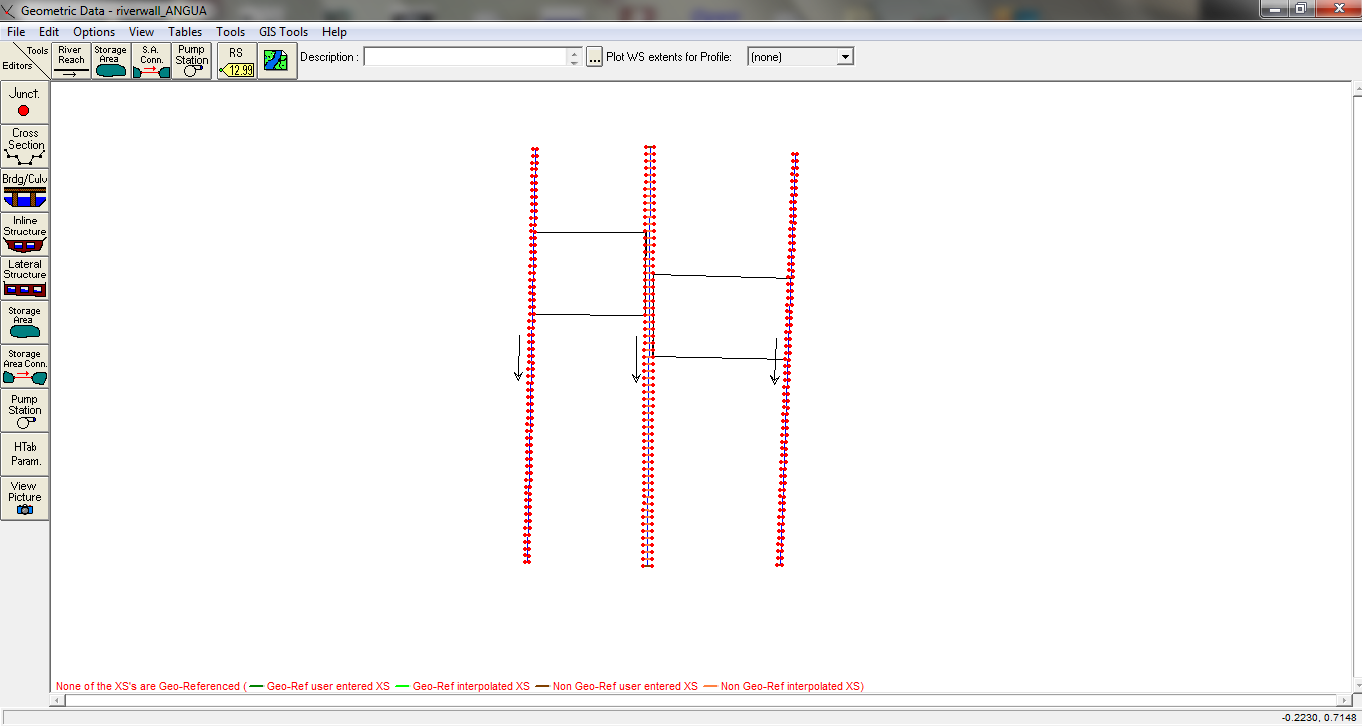
\includegraphics[width=0.9\textwidth]{hecras_riverwall_anugaTest/RASGeometry_levee.png}
\end{center}
\caption{HECRAS model geometric schematization. The `right' channel appears on
the left side of this figure, and the `left' on the right.}
\label{schematic}
\end{figure}

A HECRAS model was set up with 3 uniform parallel channels (`left', `middle',
`right', orientations defined when looking downstream). All channels had
lengths of 1000m, bed-slope $3/1000$, manning's n of 0.03, while their widths were 10m,
20m, and 10m respectively (Figure~\ref{schematic}). The cross-sections were all
nearly-flat (three-points with bank elevations 1cm above the central bed
elevation), and for all reaches the most upstream cross-section (1000) had an
elevation of 0m. These three channels were connected with broad-crested lateral
weirs (using HecRAS's default lateral weir drag coefficient of 1.1 in metric
units). The `right' and `middle' channels were connected with a 198m long weir
with an elevation 0.5m above the bed, from stations 799 to 601. The `left' and
'middle' channels were connected with a 198m long weir with an elevation 0.5m
above the bed from stations 699 to 501. 

Throughout the simulation the `left' and `right' channels were given a
discharge of 0.1m$^3$/s (just enough to prevent them drying, which causes numerical
blow-up in in HECRAS). The `middle' channel was given a discharge timeseries,
increasing from 1m$^3$/s to 21m$^3$/s over a few hours of simulated time. The entire model
is run for 24hours.

As the discharge in the central channel increases, water starts to overtop the
riverwalls and flows into the side channels. The loss/gain and final
equilibrium flow state in each channel is determined by the flow over the
riverwalls, which is itself a function of the stage in each river. Although
both riverwalls are 0.5m above the bed, the `right' channel receives more water
than the `left' channel because it has the most upstream connection to the
`middle' channel. Further downstream the `middle' channel has already lost a
significant part of its discharge, so it flows less deeply and there is less flux over
the more downstream riverwall.

An analagous ANUGA model was set up with riverwalls connecting 3 channels.
The Qfactor for both riverwalls was set to (1.1/1.7$\simeq$0.65) to make the ANUGA
riverwall drag coefficient equivalent to the default HECRAS drag coefficient. The
same discharge timeseries, elevations, and manning's n values were used. The
initial conditions in each model are slightly different but this is only
important in the first hour of simulation.

\subsection{Results}

Figures~\ref{midReach}-\ref{leftReach} show stage timeseries at various
stations downstream in each channel. The results are qualitatively similar,
with stages typically differing by a few cm. The main exception is in areas
just upstream of the weir (800 on the right channel, 700 on the left), where
HECRAS predicts a greater a backwater effect in the receiving channel than
ANUGA. This may be because of differences in the transport of momentum over the
riverwall. HECRAS apparently only transfers mass (??), whereas ANUGA transfers
both mass and momentum. This could cause more stagnation at the upstream parts
of the riverwall overflow in HECRAS, since the water is transferred to the side
channels without a downstream component of momentum.

We do not expect exact similarity because ANUGA's model is different to the
HECRAS [e.g. in the transfer of momentum over riverwalls, riverwall submergence
correction, different numerics, 1D vs 2D]. Also, there are some limitations in
the numerics of this HECRAS model that should be explored and fixed. For
example, uniform flow sections in the upstream parts of each HECRAS reach do
not seem to exactly get the correct uniform flow solution based on Manning's
equation, although they are close. We expect these limitations are with our
HECRAS model setup (we didn't adjust the solver's default numerical options)
rather than being intrinsic to the software. 

Irrespective, the main point of this comparison is that both ANUGA and HecRAS
are giving similar results for this case study, even though their underlying
models are different.


\begin{figure}
\begin{center}
\includegraphics[width=0.9\textwidth]{MIDDLE_REACH.png}
\end{center}
\caption{Stage at various points downstream in the middle channel}
\label{midReach}
\end{figure}

\begin{figure}
\begin{center}
\includegraphics[width=0.9\textwidth]{RIGHT_REACH.png}
\end{center}
\caption{Stage at various points downstream in the right channel}
\end{figure}

\begin{figure}
\begin{center}
\includegraphics[width=0.9\textwidth]{LEFT_REACH.png}
\end{center}
\caption{Stage at various points downstream in the left channel}
\label{leftReach}
\end{figure}


\endinput
